\subsection{Functions}\label{subsec-functions}

\begin{definition}\label{def-function}
    Let $M,N$ be two sets. A subset $F \subset M \times N$ is called a function
    from $M$ to $N$ if \cite[p.27]{wuest2009}
    \begin{equation}
        (\left<x,y\right> \in F \land \left<x,z\right> \in F) 
        \implies y = z \quad (x \in M,\:y,z \in N)
    \end{equation}
\end{definition}

\begin{definition}\label{def-domain-range}
    Let $F \subset M \times N$ be a function. The sets
    \begin{align}
        \domain{F} &= \left\{x \setbuild x \in M \text{ there exists } y \in N \text{ with } \left<x,y\right> \in F \right\} \label{def-domain}\\
        \codomain{F} &= \left\{y \setbuild y \in N \text{ there exists } x \in M \text{ with } \left<x,y\right> \in F \right\} \label{def-codomain}
    \end{align}
    are called domain and codomain, respectively.
\end{definition}

\begin{figure}[ht!]
    \centering
    \begin{tikzpicture}
        % center rectangle
        \draw [color=black,dashed] (0,0) rectangle (6,4) node[above] {$X \times Y$};
        \draw [color=red,very thick] (1,1) to[out=-45,in=180] (5,3) node[below,anchor=south east] {$F\subset M \times N$};
        % horizontal bar
        \draw [color=MidnightBlue,very thick] (0,-1) -- (6,-1) node[anchor=north east] {$X$};
        \draw [color=BurntOrange,very thick] (1,-1) -- (5,-1) node[anchor=north east] {$F^{-1}(N)$}; 
        \draw [color=BurntOrange,dashed] (1,-1) -- (1,1);
        \draw [color=BurntOrange,dashed] (5,-1) -- (5,3);
        % vertical bar
        \draw [color=DarkOrchid,very thick] (-1,0) -- (-1,4) node[anchor=north east] {$Y$};
        \draw [color=ForestGreen,very thick] (-1,1) -- (-1,3) node[anchor=north east] {$F(M)$};  
        \draw [color=ForestGreen,dashed] (-1,1) -- (1,1);  
        \draw [color=ForestGreen,dashed] (-1,3) -- (5,3);    
    \end{tikzpicture}
    \caption{Graphical depiction of a valid sample function}
    \label{sketch-valid-function}
\end{figure}

\begin{flushleft}
    If $\domain{F}\subset M$ with $F$ as a well defined function, we will use the
    the following shorthand notations as is customary:
    \begin{align*}
        F:\;&\mathcal{D} \rightarrow N\\
          &x\mapsto F(x)\\\\
        \text{or}\quad&F:x\mapsto F(x)\qquad{(x\in\mathcal{D})}\\\\
        \text{or}\quad&F:y=F(x)\qquad{(x\in\mathcal{D})}
    \end{align*}
\end{flushleft}

\begin{definition}\label{def-image-preimage}
    Let $F : X \rightarrow Y$ be a function where $M\subseteq X$ and $N \subseteq Y$.
    Then
    \begin{align}
        F(M) &\defines \left\{F(x) \setbuild x \in M \right\}\subseteq Y \label{eq-image} \\
        F^{-1}(N) &\defines \left\{x \in X \setbuild F(x) \in N \right\}\label{eq-preimage}
    \end{align}
    are called the image\footnote{Alternative notation: $\text{Im}(F)$} of $M$ 
    under $F$ and the preimage\footnote{Urbild (\textit{German})} of $F$ under $N$, respectively 
    \cite[p.16]{liesenMehrmann2015}.
\end{definition}

\begin{rem}
    The domain can be any arbitrary set that makes sense for a function $F$ (e.g.
    don't allow dividing by zero). The image is the set of all possible values the
    function can actually take on. Often the codomain is equal to the image of a
    function, but in some instances this is not the case. For example,
    \begin{align*}
        F(x):\mathbb{R}\rightarrow\mathbb{R},x\mapsto x^2
    \end{align*}
    In this example $F(x)\defines x^2$ can never take on any negative numbers, 
    so the image of $F$ is $F(\mathbb{R})=[0,\infty)\subset\domain{F}$. This 
    function never assumes any negative numbers which clearly also belong to the
    set of real numbers. On the other hand, the preimage of the image should be 
    the whole domain. Each subset of the image has a preimage that can be considered
    separately, e.g. $ F^{-1}(\{4,9\})=\{-3,-2,2,3\}$. 
\end{rem}

\begin{figure}[ht!]
    \centering
    \begin{tikzpicture}
        % center rectangle
        \draw [color=black,dashed] (0,0) rectangle (6,4) node[above] {$X \times Y$};
        \draw [color=red,very thick] (1,1) to[out=-50,in=20] (1,3) node[below,anchor=south west] {$F\subset M \times N$};
        % horizontal bar
        \draw [color=MidnightBlue,very thick] (0,-1) -- (6,-1) node[anchor=north east] {$X$};
        \draw [color=BurntOrange,very thick] (1,-1) -- (5,-1) node[anchor=north east] {$F^{-1}(N)$}; 
        \draw [color=BurntOrange,dashed] (1,-1) node[anchor=south west] {$x$} -- (1,3);
        % vertical bar
        \draw [color=DarkOrchid,very thick] (-1,0) -- (-1,4) node[anchor=north east] {$Y$};
        \draw [color=ForestGreen,very thick] (-1,1) -- (-1,3) node[anchor=north east] {$F(M)$};  
        \draw [color=ForestGreen,dashed] (-1,1) node[anchor=north west] {$y_1$} -- (1,1);
        \draw [color=ForestGreen,dashed] (-1,3) node[anchor=north west] {$y_2$} -- (1,3);
    \end{tikzpicture}
    \caption{Example of what constitutes a violation of \pref{definition}{def-function}}
    \label{sketch-invalid-function}
\end{figure}

\begin{definition}
    Let $F \subset M \times N$ be a function from $M$ to $N$ $:\Leftrightarrow \domain{F}=M$.
    Then for $x_1,x_2\in M, y\in N$:
    \begin{itemize}
        \item $F$ surjective $:\Leftrightarrow\codomain{F}=N$\label{def-surjective}
        \item $F$ injective $:\Leftrightarrow(\left<x_1,y\right>\in F \land \left<x_2,y\right>\in F)\implies x_1=x_2$\label{def-injective}
        \item $F$ bijective $:\Leftrightarrow$ $F$ surjective and injective \label{def-bijective}
    \end{itemize}
\end{definition}

\begin{exm}\label{exm-injective-function}
    Let $f:\mathbb{R}\rightarrow\mathbb{R},f(x)=2x+3$. Is this function injective?
    \begin{flushleft}
        \textbf{Answer}: Suppose there are two values $x_1,x_2\in\mathbb{R}$ such
        that $f(x_1)=f(x_2)$. Then
        \begin{align*}
                     f(x_1) &= f(x_2) \\
            \implies 2x_1+3 &= 2x_2+3 \\
            \implies   2x_1 &= 2x_2   \\
            \implies    x_1 &= x_2
        \end{align*}
        Therefore the function $f(x)=2x+3$ is injective. With respect to
        \pref{figure}{sketch-injective-function} this means that every value from
        the codomain is taken on \textit{at most} once.
    \end{flushleft}
    \begin{rem}
        In order to determine whether a function is injective 
        or not assume that there exists an $x_1,x_2$ where $x_1 \neq x_2$ such
        that $f(x_1)=f(x_2)$. If you can show that this is only true for $x_1=x_2$
        then you are done, if not then the function is not injective. 
    \end{rem}
\end{exm}

\begin{figure}[ht!]
    \centering
    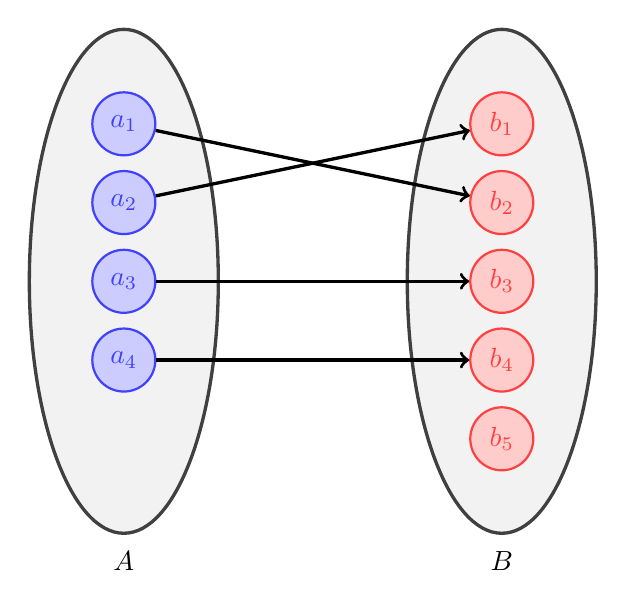
\begin{tikzpicture}[scale=0.8]
        \tikzstyle{blue-node}=[color=blue!75,fill=blue!20,thick,circle, draw, minimum width=0.8cm]
        \tikzstyle{red-node}=[color=red!75,fill=red!20,thick,circle, draw, minimum width=0.8cm]
        \tikzstyle{parent}=[color=black!75,fill=black!5,very thick]
        \tikzstyle{mapsto}=[->,very thick]
        % set A
        \draw [parent] (-2,0) ellipse (1.5cm and 4cm);       
        \node [blue-node] at (-2,2.5) (a1) {$a_1$};        
        \node [blue-node] at (-2,1.25) (a2) {$a_2$};
        \node [blue-node] at (-2,0) (a3) {$a_3$};
        \node [blue-node] at (-2,-1.25) (a4) {$a_4$} (-2,-4.75) node[anchor=south,color=black] {$A$};
        % set B
        \draw [parent] (4,0) ellipse (1.5cm and 4cm);
        \node [red-node] at (4,2.5) (b1) {$b_1$};
        \node [red-node] at (4,1.25) (b2) {$b_2$};
        \node [red-node] at (4,0)(b3) {$b_3$};
        \node [red-node] at (4,-1.25) (b4) {$b_4$};
        \node [red-node] at (4,-2.5) (b5) {$b_5$} (4,-4.75) node[anchor=south,color=black] {$B$};
        % mapsto
        \draw [mapsto] (a1) -- (b2);
        \draw [mapsto] (a2) -- (b1);
        \draw [mapsto] (a3) -- (b3);
        \draw [mapsto] (a4) -- (b4);
    \end{tikzpicture}
    \caption{Example of an injective function}
    \label{sketch-injective-function}
\end{figure}

\begin{exm}\label{exm-surjective-function}
    Let $f:\mathbb{R}\rightarrow\mathbb{R},f(x)=2x+3$. Is this function surjective?
    \begin{flushleft}
        \textbf{Answer}: For any $y=f(x)\in\mathbb{R}$ there exists an $x=\frac{y-3}{2}$
        such that
        \begin{align*}
            f(x) &= 2\left(\frac{y-3}{2}\right)+3 \\
                 &= y - 3 + 3 \\
                 &= y
        \end{align*}
        This proves that the function $f(x)=2x+3$ is surjective since $\text{Im}(f)=\mathbb{R}$. 
        With respect to \pref{figure}{sketch-surjective-function} this means that 
        every value from the codomain is taken on \textit{at least} once.
    \end{flushleft}
    \begin{rem}
        The strategy for determining whether a function is 
        surjective or not boils down to solving the original function definition
        for $x$ and plugging in this expression in $f(x)$. If you can show that 
        $f(x)=y$ then you are done, if not then the function is not surjective.
    \end{rem}
\end{exm}

\begin{figure}[ht!]
    \centering
    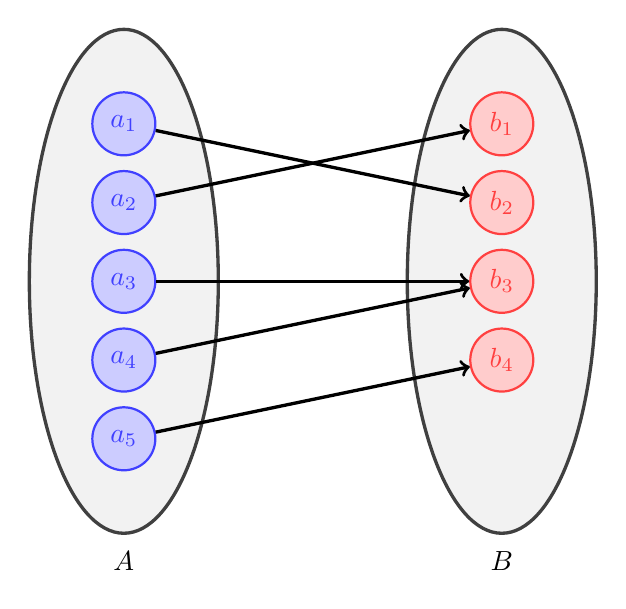
\begin{tikzpicture}[scale=0.8]
        \tikzstyle{blue-node}=[color=blue!75,fill=blue!20,thick,circle, draw, minimum width=0.8cm]
        \tikzstyle{red-node}=[color=red!75,fill=red!20,thick,circle, draw, minimum width=0.8cm]
        \tikzstyle{parent}=[color=black!75,fill=black!5,very thick]
        \tikzstyle{mapsto}=[->,very thick]
        % set A
        \draw [parent] (-2,0) ellipse (1.5cm and 4cm);       
        \node [blue-node] at (-2,2.5) (a1) {$a_1$};        
        \node [blue-node] at (-2,1.25) (a2) {$a_2$};
        \node [blue-node] at (-2,0) (a3) {$a_3$};
        \node [blue-node] at (-2,-1.25) (a4) {$a_4$};
        \node [blue-node] at (-2,-2.5) (a5) {$a_5$} (-2,-4.75) node[anchor=south,color=black] {$A$};
        % set B
        \draw [parent] (4,0) ellipse (1.5cm and 4cm);
        \node [red-node] at (4,2.5) (b1) {$b_1$};
        \node [red-node] at (4,1.25) (b2) {$b_2$};
        \node [red-node] at (4,0)(b3) {$b_3$};
        \node [red-node] at (4,-1.25) (b4) {$b_4$} (4,-4.75) node[anchor=south,color=black] {$B$};
        % mapsto
        \draw [mapsto] (a1) -- (b2);
        \draw [mapsto] (a2) -- (b1);
        \draw [mapsto] (a3) -- (b3);
        \draw [mapsto] (a4) -- (b3);
        \draw [mapsto] (a5) -- (b4);
    \end{tikzpicture}
    \caption{Example of an surjective function}
    \label{sketch-surjective-function}
\end{figure}

\begin{exm}\label{exm-bijective-function}
    Let $f:\mathbb{R}\rightarrow\mathbb{R},f(x)=2x+3$. Is this function bijective?
    \begin{flushleft}
        \textbf{Answer}: From \pref{example}{exm-injective-function} and
        \pref{example}{exm-surjective-function} we can deduce that since the function
        is injective and surjective, that it is bijective as well. With respect 
        to \pref{figure}{sketch-bijective-function} this means that every value 
        from the codomain is taken on \textit{exactly} once.
    \end{flushleft}
\end{exm}

\begin{figure}[ht!]
    \centering
    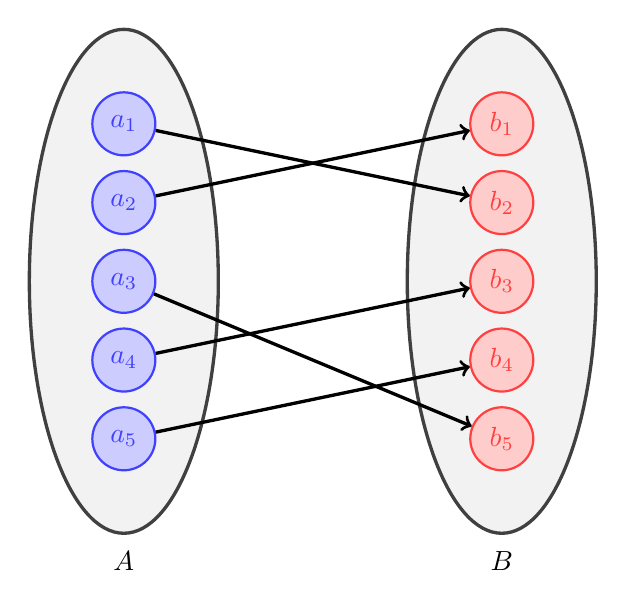
\begin{tikzpicture}[scale=0.8]
        \tikzstyle{blue-node}=[color=blue!75,fill=blue!20,thick,circle, draw, minimum width=0.8cm]
        \tikzstyle{red-node}=[color=red!75,fill=red!20,thick,circle, draw, minimum width=0.8cm]
        \tikzstyle{parent}=[color=black!75,fill=black!5,very thick]
        \tikzstyle{mapsto}=[->,very thick]
        % set A
        \draw [parent] (-2,0) ellipse (1.5cm and 4cm);       
        \node [blue-node] at (-2,2.5) (a1) {$a_1$};        
        \node [blue-node] at (-2,1.25) (a2) {$a_2$};
        \node [blue-node] at (-2,0) (a3) {$a_3$};
        \node [blue-node] at (-2,-1.25) (a4) {$a_4$};
        \node [blue-node] at (-2,-2.5) (a5) {$a_5$} (-2,-4.75) node[anchor=south,color=black] {$A$};
        % set B
        \draw [parent] (4,0) ellipse (1.5cm and 4cm);
        \node [red-node] at (4,2.5) (b1) {$b_1$};
        \node [red-node] at (4,1.25) (b2) {$b_2$};
        \node [red-node] at (4,0)(b3) {$b_3$};
        \node [red-node] at (4,-1.25) (b4) {$b_4$};
        \node [red-node] at (4,-2.5) (b5) {$b_5$} (4,-4.75) node[anchor=south,color=black] {$B$};
        % mapsto
        \draw [mapsto] (a1) -- (b2);
        \draw [mapsto] (a2) -- (b1);
        \draw [mapsto] (a3) -- (b5);
        \draw [mapsto] (a4) -- (b3);
        \draw [mapsto] (a5) -- (b4);
    \end{tikzpicture}
    \caption{Example of an bijective function}
    \label{sketch-bijective-function}
\end{figure}

\begin{exm}\label{exm-injective-surjective-bijective}
    Determine whether the following functions are injective, surjective or
    bijective\footnote{You may also consult \pref{figure}{sktech:exm-1:4} for
    additional help.}:
    \begin{enumerate}
        \item[1.)] $f(x):\mathbb{R}^+\rightarrow\mathbb{R}^+,x\mapsto x^2-1$
        \item[2.)] $g(x):\mathbb{R}^+\rightarrow\mathbb{R},x\mapsto x^2-1$
        \item[3.)] $h(x):\mathbb{R}\rightarrow\mathbb{R}^+,x\mapsto x^2-1$
        \item[4.)] $i(x):\mathbb{R}\rightarrow\mathbb{R},x\mapsto x^2-1$ 
    \end{enumerate}
    \begin{flushleft}
        \textbf{Answer:} TODO
    \end{flushleft}
\end{exm}

\begin{definition}\label{def-inverse-function}
    Let $f:\mathcal{D}\to\mathcal{C}$. We say that $f$ is invertible if there exists
    $f^{-1}:\mathcal{C}\to\mathcal{D}$ such that
    \begin{equation}
        \forall x\in\mathcal{D}:(f^{-1}\circ f)(x)=x 
        \land \forall y\in\mathcal{C}:(f \circ f^{-1})(y)=y
    \end{equation}
    If that's the case, we call $f^{-1}$ the inverse function of $f$.
\end{definition}

\begin{thm}\label{thm-inverse-function}
    A function $f$ is invertible, \textit{iff} it is bijective.
\end{thm}

\begin{rem}\label{rem-sqrt-function}
    In school we learnt that the function 
    \begin{equation}\label{eq-sqrt-function}
        f:\mathbb{R}^+\to\mathbb{R}^+,x\mapsto\sqrt{x}
    \end{equation}
    is the inverse function of
    \begin{equation}\label{eq-pow-function}
        f:\mathbb{R}\to\mathbb{R}^+,x\mapsto x^2
    \end{equation}
    Notice that the square root function in \pref{equation}{eq-sqrt-function} is 
    only defined for positive values on $\mathbb{R}$. This is because the principal
    square root is positive:
    \begin{equation}\label{eq-sqrt-abs-function}
        \sqrt{x^2}=\abs{x}
    \end{equation}
    You may have been taught in physics that the square root function can take on
    two values, \textit{i.e.} $\sqrt{x^2}=\pm x$, for example
    \begin{equation*}
        f(x=9)=\sqrt{9}\implies x=3 \lor x=-3
    \end{equation*}
    But \pref{theorem}{thm-inverse-function} states that inverse functions are 
    bijective\footnote{To satisfy this old notion, the square root function would
    have to be strictly surjective, see also \pref{figure}{sketch-surjective-function}.}.
    \begin{figure}[h!]
        \centering
        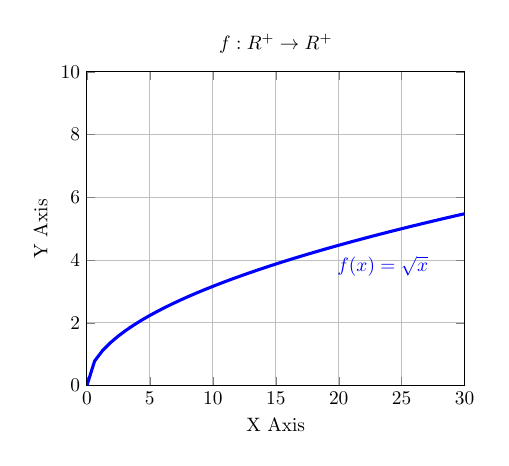
\begin{tikzpicture}[scale=0.7]
            \begin{axis}[
                xmax=30,
                xmin=0,
                ymax=10,
                ymin=0,
                samples=50,
                grid=major,
                xlabel={X Axis},
                ylabel={Y Axis},
                title={$f:\mathbb{R}^+\to\mathbb{R}^+$}
            ]
            \addplot[blue, ultra thick,domain=0:30]{sqrt(x)} node[anchor=north west,pos=0.65] {$f(x)=\sqrt{x}$};
        \end{axis}
        \end{tikzpicture}
        \caption{The square root function only operates with positive numbers}
        \label{sketch:rem-sqrt-function}
    \end{figure}
    So, while it is sometimes convenient to follow the convention in \pref{equation}{eq-sqrt-abs-function},
    strictly speaking the square root function only ever takes on positive values
    (\textit{cf.} \pref{figure}{sketch:rem-sqrt-function}).
\end{rem}

\begin{definition}\label{def-floor-function}
    The floor function is defined by
    \begin{equation}
        \ffloor(x)=\floor{x}\defines\max\left\{m\in\mathbb{Z}\setbuild m\leq x\right\}
    \end{equation}
\end{definition}

\begin{definition}\label{def-ceiling-function}
    The ceiling function is defined by
    \begin{equation}
        \fceil(x)=\ceil{x}\defines\min\left\{n\in\mathbb{Z}\setbuild n\geq x\right\}
    \end{equation}
\end{definition}

\begin{definition}\label{def-dirichlet-function}
    The Dirichlet function is defined by
    \begin{equation}
        D(x)=\begin{cases}
            1\text{ if }x\in\mathbb{Q}\\
            0\text{ else }
        \end{cases}
    \end{equation}
\end{definition}

\begin{definition}\label{def-absolute-value-function}
    The absolute value function is defined by
    \begin{equation}
        \forall x\in\mathbb{R}: \abs{x}\defines\max\{x,-x\}=\begin{cases}
            x\text{ if } x \geq 0 \\
            -x \text{ else }
        \end{cases}
    \end{equation}
\end{definition}

\begin{thm}\label{thm-absolute-value-properties}
    Below are listed some of the properties related to the absolute value; for
    any $x\in\mathbb{R}$ the following holds:
    \begin{enumerate}
        \item $\abs{x} \geq 0$
        \item $\abs{x} \geq \pm x$
        \item $\abs{x} = \abs{-x}$
        \item $\abs{x} = 0 \iff x = 0$
        \item $\abs{xy} = \abs{x}\abs{y}$
        \item $\abs{x} + \abs{y} \geq \abs{x+y}$
        \item $\abs{x-y} \geq \abs[\big]{\abs{x}-\abs{y}}$
        \item $\abs{x} < M \iff -M < x < M$
    \end{enumerate}
\end{thm}

\begin{proof}
    Of theorem (\ref{thm-absolute-value-properties}).
    \begin{flushleft}
        In this proof we will only show property 6 of this theorem which is also
        known as the triangle inequality. From property 2 it follows that the sum 
        of $\abs{x}\geq x$ and $\abs{y}\geq y$ equals
        \begin{equation}\label{tmp-absolute-value-properties:1}
            \abs{x} + \abs{y} \geq x + y
        \end{equation}
        Likewise, from $\abs{x}\geq -x$ and $\abs{y}\geq -y$ it follows that
        \begin{equation}\label{tmp-absolute-value-properties:2}
            \abs{x} + \abs{y} \geq -(x+y)
        \end{equation}
        Thus, by definition (\ref{def-absolute-value-function}) and equation
        (\ref{tmp-absolute-value-properties:1}) and (\ref{tmp-absolute-value-properties:2})
        we can conclude that
        \begin{equation*}
            \abs{x} + \abs{y} \geq \abs{x+y}
        \end{equation*}
    \end{flushleft}
\end{proof}

\begin{rem}
    A geometric interpretation of the absolute value function $\abs{x}$ is the 
    distance from $x$ to $0$. Similarly, the absolute value of the difference 
    $\abs{x-y}$ can be interpreted as the distance between $x$ and $y$. See also
    \hyperref[subsec-metric-spaces]{the subsection for metric spaces} for more 
    more information on distances.
\end{rem}
